\documentclass{article}

\usepackage{times}
%% math packages
\usepackage{amsmath}		 
\usepackage{amsfonts}	
\usepackage{mathrsfs} % required for \mathscr
\usepackage{amssymb}
%% graphics 	 	
\usepackage{graphicx}	

%% alltt (alternative tt)
\usepackage{alltt}
\usepackage{color}
%% to include pdfs
\usepackage{pdfpages}


%% nicer tables
\usepackage{booktabs}
\usepackage{url}

\bibliographystyle{apalike}
\usepackage[round]{natbib}  % for ACL-style referencing
\usepackage[utf8]{inputenc}

\title{Improving language technology \\with fortuitous data \\\begin{small}ESSLLI 2016 advanced course\end{small}}
\author{Anders Johannsen \and Barbara Plank\and Željko Agić}
\date{}
\begin{document}
\maketitle

%\tableofcontents

%\listoffigures
%\listoftables

\begin{abstract}
In this course, we present approaches to facilitate natural language processing (NLP) development when confronted by sparsity, or even absence, of supervision through annotated, biased samples of language data. By using part-of-speech tagging and syntactic dependency parsing as running examples, we outline approaches to augmenting supervised techniques for top-level performance. The approaches include semi-supervised and unsupervised techniques, domain adaptation and cross-lingual learning. We place particular emphasis on leveraging the various sources of \textit{fortuitous data} that may be available even in the most severely under-resourced domains of natural language. We argue that fortuitous data provides often the `secret sauce' to make approaches based on limited supervision work. 

This handbook will complement the day-by-day notebooks (available from \url{https://github.com/andersjo/fortuitous-esslli}) by providing additional background and pointers to reading material.

\textcolor{magenta}{if we want to have it at all, will be most probably only a very short overview, something like our Google doc, plus additional references for the different days and some of our papers}
\end{abstract}

\section{Day 1: Introduction. The hunt for a learning signal.}


\textit{A learning analogy.} One sensible way of learning to cook an unknown dish is to find a recipe and follow the steps. Most successful machine learning approaches work in a slightly different way. They in fact carefully avoid looking at the step-to-step instructions and instead just combine the given ingredients according to the their current (pretty bad) idea of how cooking works. Finally the learners compare the end result to the picture of the dish in the recipe. It's not as crazy as it sounds. If it looks alright, they will conclude that all is well and that they already knew how to cook, and they would be right. If it?s slightly off, they would like to improve their efforts the next time around, so they think back at what they did, working out how to slightly adjust their procedure to make the end-result closer to the picture in the recipe. Comparing the result and the picture provides a learning signal. Going through many many recipes in this manner and making small adjustment to the procedures eventually means that you'll learn to cook. 

Gradient-based learning where the model makes predictions during training and is updated in a direction that makes it less wrong is ubiquitous in NLP and accounts for most successes in machine learning, including deep learning. In supervised learning the learning signal is straightforward. For every input in the training set there?s a corresponding output, which is what is what we are interested in learning. 

A couple of challenges to this model

Target function might be simple enough, but with sparse input (and words are \"uber-sparse) you are forced to obtain large amounts of data.
Labeled data set might be small, but another data set with related labels might be interesting. How to incorporate.  
Domain adaptation
Change in input distribution.
Change in relation between input and output

We will demonstrate these problems and challenges on a couple of toy problems. In the first lecture we?ll assume that both our input and output have a fixed size and structure, i.e. the problem is classification. This will also serve to motivate the structured models that are the topic of Day 2. 


\section{Day 2: Structured input and output}

\begin{itemize}
\item sequence learning, tagging, parsing
\item from traditional to deep learning (RNNs, sequence2sequence)
\end{itemize}

\section{Day 3: Hands-on, exercise day}
delving into methods and how
they tight up with fortuitous data 

overview of a plethora of possibilites, some
hand-picked examples they can work with


[ 2-3 concrete hands-on examples ] 
An inspirational catalogues of sources of learning signals.

A departure from the supervised paradigm: reinforcement learning with policy gradients.

Finish an experiment with injecting additional data into a system via Jupyter notebooks.

Possible exercises using:
Traditional structured perceptron tagger 
NN-based tagger 


\section{Day 4: Representations and Multi-task learning}


How to share representations across jointly as well as separately trained tasks. For multi-task, see Plank et al ACL 2016 + EMNLP submission (keystrokes).

What kind of representations are useful. Exploring word embeddings, and character/byte embeddings. Can a sentence be represented as a vector?



\section{Day 5: Cross-lingual learning}

Cross-lingual learning is an extreme case of adaptation: learning when there is no annotated data to start off with.


See Agic et al. 2015 ACL (tagging), 2016 TACL (parsing), 2016 ACL (ILP), 2016 EMNLP (evaluation)

\clearpage
\pagenumbering{gobble}
\section{Appendix: selected papers}

\begin{itemize}
\item Plank et al. (2016). \textit{Multilingual Part-of-Speech Tagging with Bidirectional Long Short-Term Memory Models and Auxiliary Loss}. In ACL 2016.
\item Agić et al. (2016). \textit{Multilingual Projection for Parsing Truly Low-Resource Languages}. In TACL.
\end{itemize}
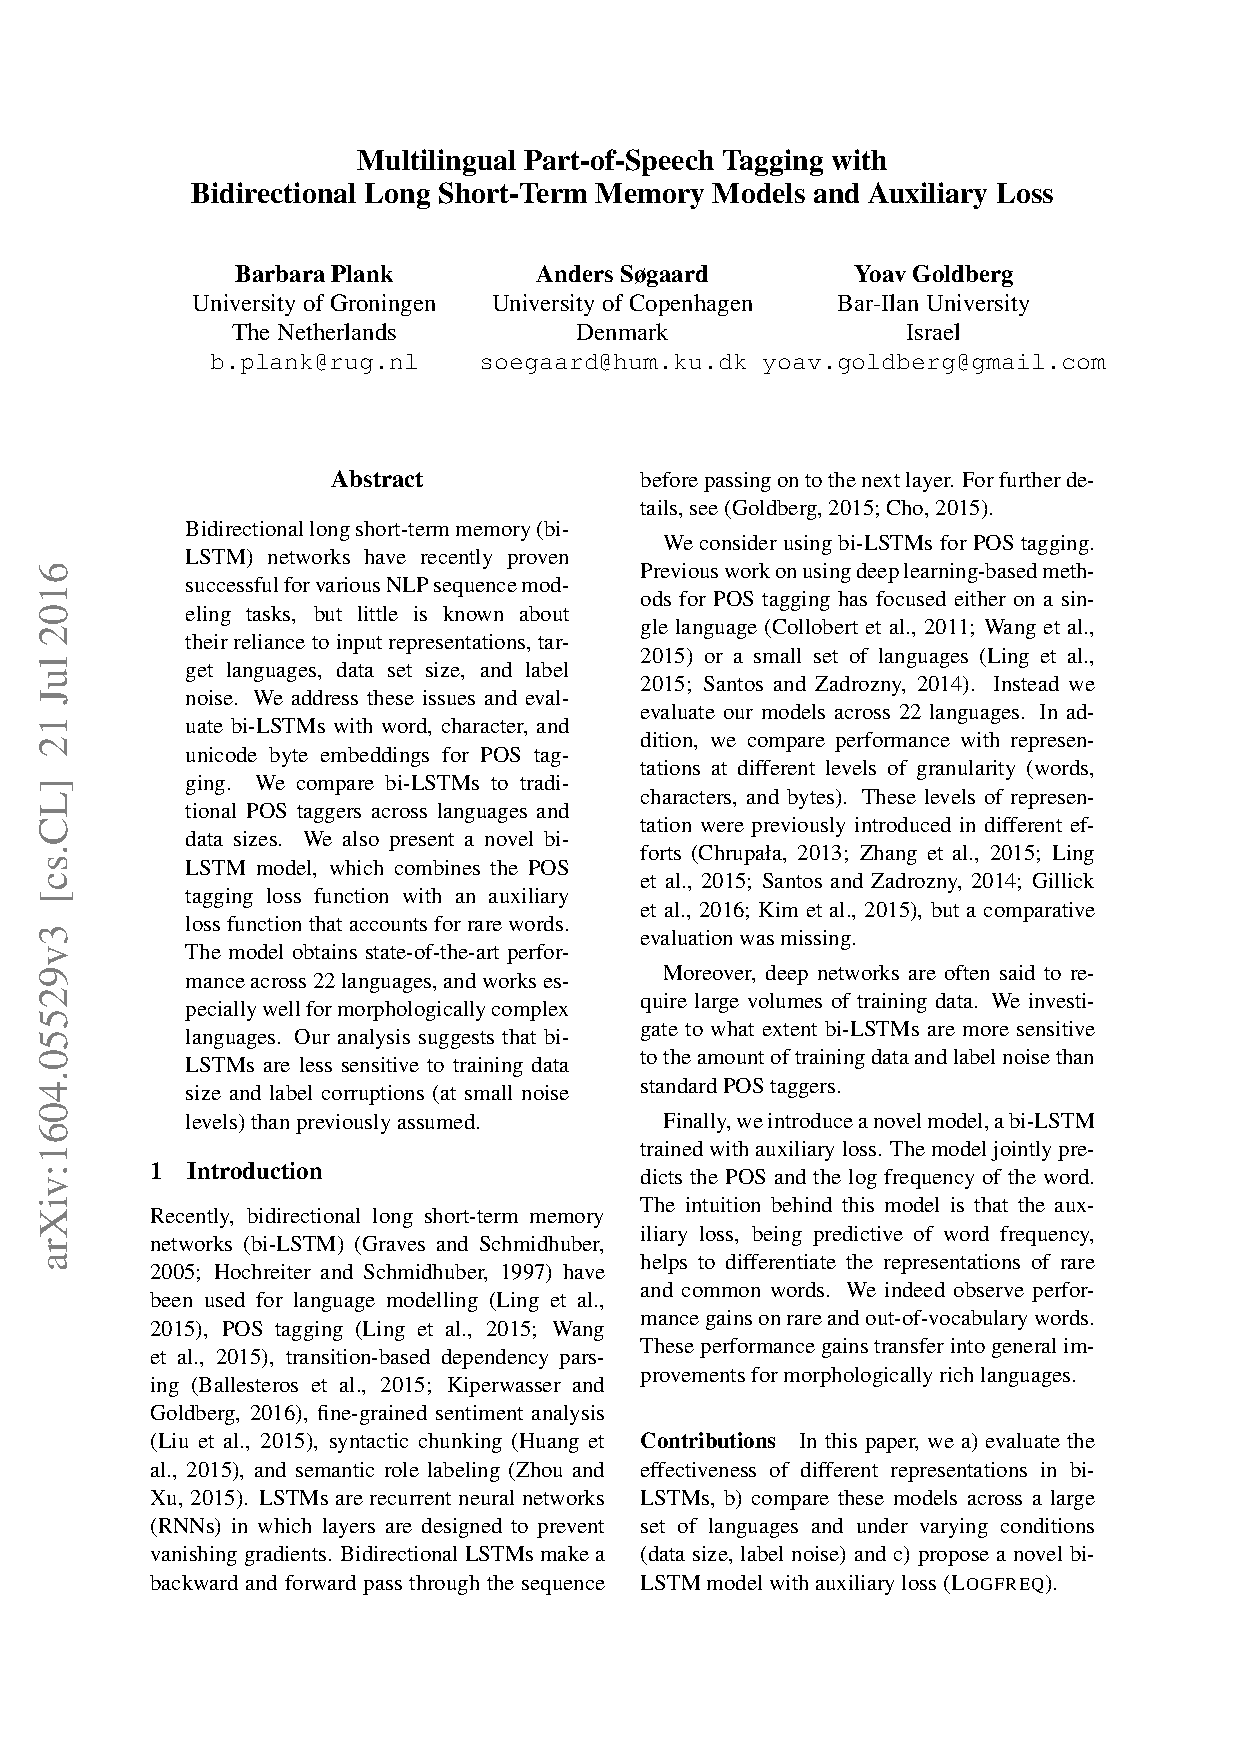
\includepdf[scale=0.9,pages=-,pagecommand=\thispagestyle{plain}]{bilstm-aux.pdf} 
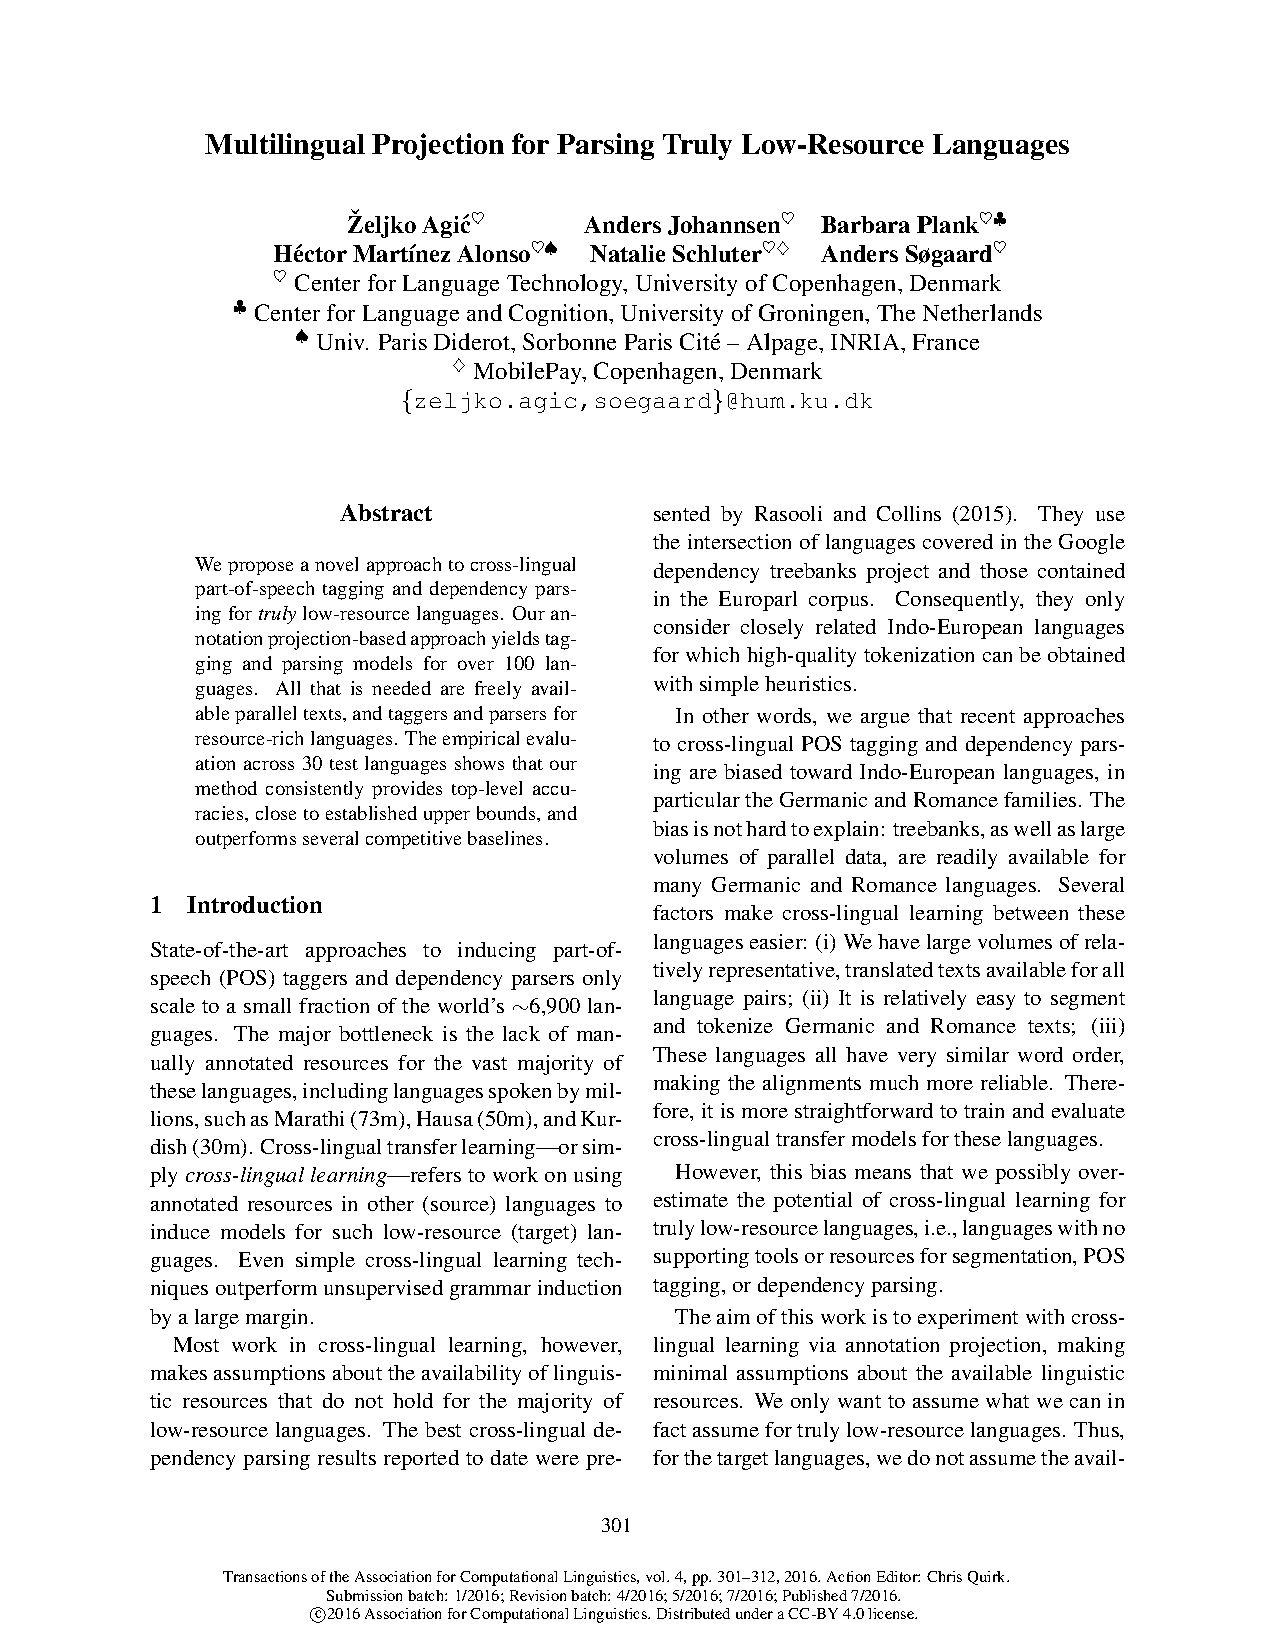
\includepdf[scale=0.9,pages=-,pagecommand=\thispagestyle{plain}]{TACL2016.pdf} 


%\clearpage
%\citep{durrett2015neural}
%\citet{durrett2015neural}

\bibliography{book}
\end{document}